\begin{frame}[c]
    \frametitle{使用微环谐振器的腔增强片上[测量]吸收光谱}
    \begin{itemize}
        \item Nitkowski, A.;  Chen, L.; Lipson, M., Cavity-enhanced on-chip \textcolor{purple}{absorption spectroscopy} using \textcolor{red}{microring resonators}. Optics Express 2008, 16 (16), 11930-11936.
        \item \textcolor{blue}{创新点:}使用环形谐振器,既保留了长光路,又减小了器件尺寸。
        \item \textcolor{blue}{意义:}微环谐振器可以有效地用于增加小型化片上器件的灵敏度。
        \item \textcolor{blue}{瓶颈:}仪器的信噪比仍然不够理想。
        \item \textcolor{blue}{原理:}利用环形谐振器延长光路,根据入射光谱、出射光谱和探测器接收光谱得到物质的吸收光谱。
    \end{itemize}
    \begin{columns}
        \begin{column}{.5\textwidth}
            仪器(部分)结构示意图:
            \begin{figure}[H] %H为当前位置,!htb为忽略美学标准,htbp为浮动图形
                \centering %图片居中
                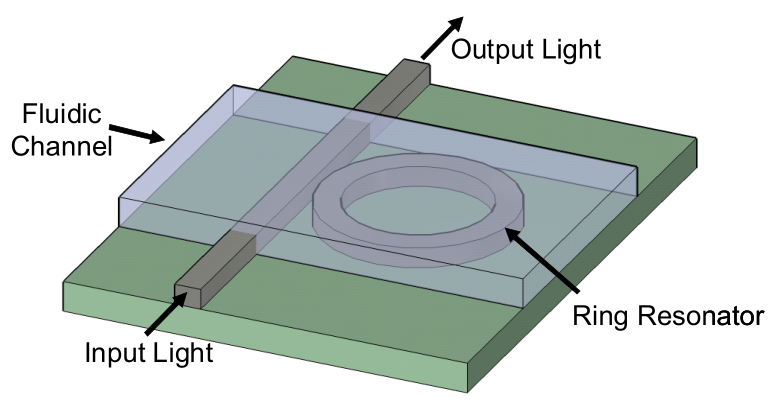
\includegraphics[width=1.\textwidth]{figures/Cavity-enhanced on-chip absorption spectroscopy using microring resonators_1.png} %插入图片,[]中设置图片大小,{}中是图片文件名
            \end{figure}
            (待测物质是液体)
        \end{column}
        \begin{column}{.5\textwidth}
            仪器原理示意图:
            \begin{figure}[H] %H为当前位置,!htb为忽略美学标准,htbp为浮动图形
                \centering %图片居中
                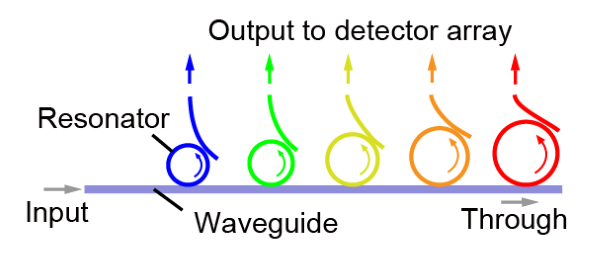
\includegraphics[width=1.\textwidth]{figures/Cavity-enhanced on-chip absorption spectroscopy using microring resonators_2.png} %插入图片,[]中设置图片大小,{}中是图片文件名
            \end{figure}
        \end{column}
    \end{columns}
\end{frame}

\begin{frame}[c]
    \frametitle{使用微环谐振器的腔增强片上[测量]吸收光谱}
    实验步骤:
    \begin{enumerate}
        \item 不注入待测物质,测量仪器固有损耗。
        \item 注入待测物质 N-methylaniline(N-甲基苯胺),测量其吸收光谱。
    \end{enumerate}
    过程细节:
    \begin{itemize}
        \item 两次实验中,入射光源分别从 1460 nm 调节到 1610 nm,步长为 1 nm。
        \item 选择该物质是因为其中的 N-H 键的吸收峰在 1500 nm 附近。
    \end{itemize}
    实验结果:
    \begin{figure}[H] %H为当前位置,!htb为忽略美学标准,htbp为浮动图形
        \centering %图片居中
        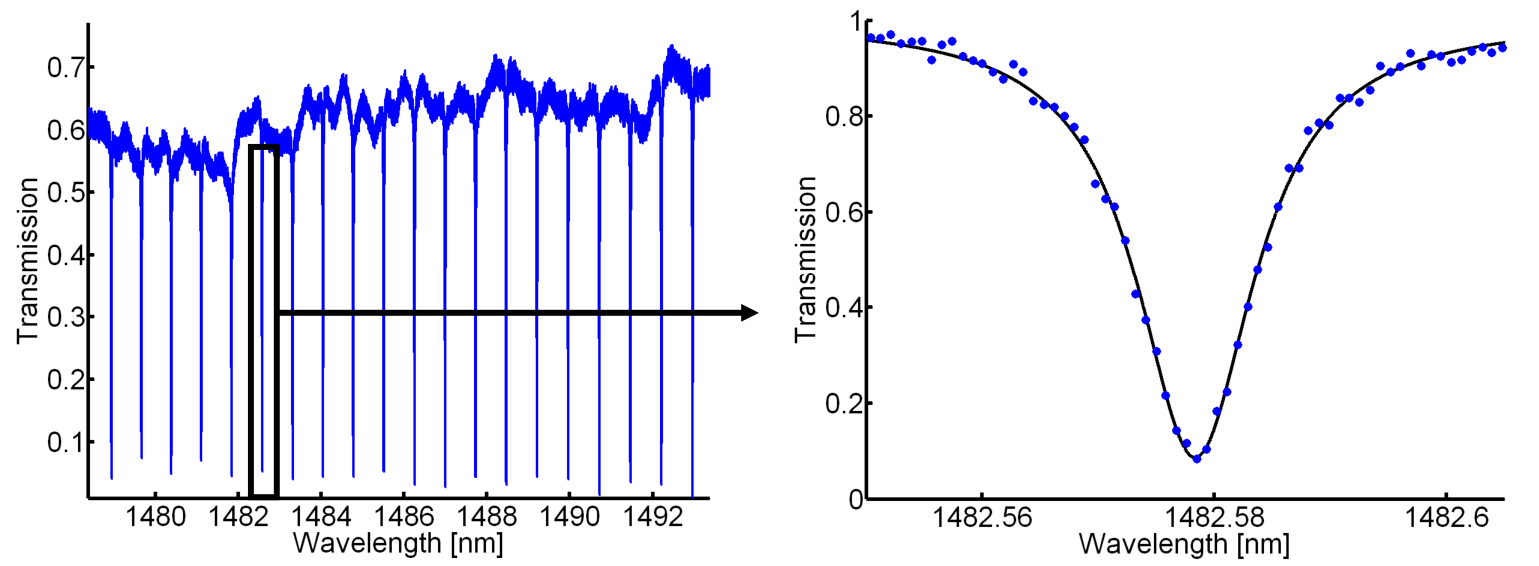
\includegraphics[width=1.\textwidth]{figures/Cavity-enhanced on-chip absorption spectroscopy using microring resonators_3.png} %插入图片,[]中设置图片大小,{}中是图片文件名
    \end{figure}
    文中还将该仪器的结果与一商用仪器相比较,两者有很好的一致性。
\end{frame}